%
% Copyright 2018 Joel Feldman, Andrew Rechnitzer and Elyse Yeager.
% This work is licensed under a Creative Commons Attribution-NonCommercial-ShareAlike 4.0 International License.
% https://creativecommons.org/licenses/by-nc-sa/4.0/
%
\questionheader{ex:s3.5.1}
%%%%%%%%%%%%%%%%%%
\subsection*{\Conceptual}
%%%%%%%%%%%%%%%%%%


\begin{Mquestion}
Identify every critical point and every singular point of $f(x)$ shown on the graph below.\\
 Which correspond to local extrema?
\begin{center}\begin{tikzpicture}
\YEaaxis{4}{4}{1}{4}
\draw[thick] plot[domain=-2.5:2](\x,{\x*\x*\x/4+2});
\draw[thick] plot[domain=2:2.5](\x,{3*(\x-3)*(\x-3)+1});
\draw[thick] plot[domain=2.5:3.1](\x,{exp(-4*(\x-2.43))+1}) node[ right]{$y=f(x)$};
\end{tikzpicture}\end{center}
\end{Mquestion}
\begin{hint}
Estimate $f'(0)$.
\end{hint}
\begin{answer}
\begin{center}\begin{tikzpicture}
\YEaaxis{4}{4}{1}{4}
\draw[thick] plot[domain=-2.5:2](\x,{\x*\x*\x/4+2});
\draw[thick] plot[domain=2:2.5](\x,{3*(\x-3)*(\x-3)+1});
\draw[thick] plot[domain=2.5:3.1](\x,{exp(-4*(\x-2.43))+1}) node[ right]{$y=f(x)$};
\draw[red] (2,4) node[vertex]{};
\draw[blue] (0,2) node[vertex]{};
\draw[thick, blue ] (0,.2)--(0,-.2);
\draw[thick, red ] (2,.2)--(2,-.2);
\end{tikzpicture}\end{center}
There is a critical point at $x=0$. The $x$-value of the red dot is a singular point, and a local maximum occurs there.
\end{answer}
\begin{solution}
\begin{center}\begin{tikzpicture}
\YEaaxis{4}{4}{1}{4}
\draw[thick] plot[domain=-2.5:2](\x,{\x*\x*\x/4+2});
\draw[thick] plot[domain=2:2.5](\x,{3*(\x-3)*(\x-3)+1});
\draw[thick] plot[domain=2.5:3.1](\x,{exp(-4*(\x-2.43))+1}) node[ right]{$y=f(x)$};
\draw[red] (2,4) node[vertex]{};
\draw[blue] (0,2) node[vertex]{};
\draw[thick, blue ] (0,.2)--(0,-.2);
\draw[thick, red ] (2,.2)--(2,-.2) node[below]{$a$};
\end{tikzpicture}\end{center}
When $x=0$, the curve $y=f(x)$ appears to have a flat tangent line, so the $x=0$ is a critical point. However, it is not a local extremum: it is not true that $f(0) \geq f(x)$ for all $x$ near 0, and it is not true that $f(0) \leq f(x)$ for all $x$ near 0.

To the right of the $x$-axis, there is a spike where the derivative of $f(x)$ does not exist. The $x$-value corresponding to this spike (call it $a$) is a singular point, and $f(x)$ has a local maximum at $x=a$.
\end{solution}


\begin{Mquestion}
Identify every critical point and every singular point of $f(x)$
on the graph below. Which correspond to local extrema? Which correspond to global extrema over the interval shown?

\begin{center}\begin{tikzpicture}[scale=0.8]
\YEaaxis{5}{5}{3}{8}
\draw[thick] plot[domain=-5:1](\x,{-(\x*1.1+5)*(\x-2)*(\x-2)/8+4});
\draw (-5,7) node[vertex]{};
\draw (1,3.25) node[opendot]{};
\draw[thick] plot[domain=1:5](\x,{-\x/4+2}) node[ above right]{$y=f(x)$};
\draw (1,1.75) node[vertex]{};
\draw (5,.75) node[vertex]{};
\end{tikzpicture}\end{center}

\end{Mquestion}
\begin{hint}
If the graph is discontinuous at a point, it is not differentiable at that point.
\end{hint}
\begin{answer}
\begin{center}\begin{tikzpicture}[scale=0.8]
\YEaaxis{5}{5}{3}{8}
\draw[thick] plot[domain=-5:1](\x,{-(\x*1.1+5)*(\x-2)*(\x-2)/8+4});
\draw (-5,7) node[vertex]{};
\draw (1,3.25) node[opendot]{};
\draw[thick] plot[domain=1:5](\x,{-\x/4+2}) node[ above right]{$y=f(x)$};
\draw (1,1.75) node[vertex]{};
\draw (5,.75) node[vertex]{};
\color{blue}
\draw (-2.36,-1.7) node[vertex]{};
\draw[thick] (-2.36,.2)--(-2.36,-.2) node[below]{$a$};
\color{red}
\draw[thick] (1,.2)--(1,-.2) node[below]{$b$};
\end{tikzpicture}\end{center}
The $x$-coordinate corresponding to the blue dot (let's call it $a$) is a critical point, and $f(x)$ has a local and global minimum at $x=a$. The $x$-coordinate corresponding to the discontinuity (let's call it $b$) is a singular point, but there is no a global or local extremum at $x=b$.
\end{answer}
\begin{solution}
\begin{center}\begin{tikzpicture}[scale=0.8]
\YEaaxis{5}{5}{3}{8}
\draw[thick] plot[domain=-5:1](\x,{-(\x*1.1+5)*(\x-2)*(\x-2)/8+4});
\draw (-5,7) node[vertex]{};
\draw (1,3.25) node[opendot]{};
\draw[thick] plot[domain=1:5](\x,{-\x/4+2}) node[ above right]{$y=f(x)$};
\draw (1,1.75) node[vertex]{};
\draw (5,.75) node[vertex]{};
\color{blue}
\draw (-2.36,-1.7) node[vertex]{};
\draw[thick] (-2.36,.2)--(-2.36,-.2) node[below]{$a$};
\color{red}
\draw[thick] (1,.2)--(1,-.2) node[below]{$b$};
\end{tikzpicture}\end{center}
The $x$-coordinate corresponding to the blue dot (let's call it $a$) is a critical point, because the tangent line to $f(x)$ at $x=a$ is horizontal. There is no lower point nearby, and actually no lower point on the whole interval shown, so $f(x)$ has both a local minimum and  a global minimum at $x=a$.

If a function is not continuous at a point, then it is not differentiable at that point. So, the $x$-coordinate  corresponding to the discontinuity (let's call it $b$) is a singular point. Values of $f(x)$ immediately to the right of $b$ are lower, and values immediately to the left of $b$ are higher, so $f(x)$ has no local (or global) extremum at $x=b$.

If we wanted to know the derivative of the function at the left endpoint, we would take the derivative from the right. This looks to be some negative real number: so it exists (therefore, the left endpoint is not a singular point) and is not zero (therefore, the left endpoint is not a critical point). Endpoints \emph{can} be critical and singular points, but this one happens to be neither.

Similarly, at the right endpoint of the interval $f'(x)$ is some negative real number, so this point is neither critical nor singular.

Remark: $f(x)$ has a global maximum at the left-most endpoint of the interval. However, we do not call this a local maximum. In order for $f(x)$ to have a local maximum at $x=c$, $c$ must be strictly inside the domain of the function. In short: \emph{endpoints can't be local extrema}.


\end{solution}


\begin{question}
Draw a graph $y=f(x)$ where a $f(2)$ is a local maximum, but it is not a  global maximum.
\end{question}
\begin{hint}
Try making a little bump at $x=2$, the letting the function get quite large somewhere else.
\end{hint}
\begin{answer}
One possible answer is shown below.
\begin{center}
\begin{tikzpicture}
\YEaaxis{1.5}{3}{3}{3}
\draw[thick] plot[domain=-1:2.5](\x,{-\x*\x*(\x-2)});
\YExcoord{1.3}{2}
\end{tikzpicture}
\end{center}
\end{answer}
\begin{solution}
One possible answer is shown below.
\begin{center}
\begin{tikzpicture}
\YEaaxis{1.5}{3}{3}{3}
\draw[thick] plot[domain=-1:2.5](\x,{-\x*\x*(\x-2)});
\YExcoord{1.3}{2}
\end{tikzpicture}
\end{center}
For every $x$ in the red interval shown below, $f(2) \geq f(x)$, so $f(2)$ is a local maximum. However, the point marked with a blue dot shows that $f(x)>f(2)$ for some $x$, so $f(2)$ is not a global maximum.
\begin{center}
\begin{tikzpicture}
\draw[dotted, fill=red!20] (1,-.5) rectangle (1.75,1.5);
\YEaaxis{1.5}{3}{3}{3}
\draw[thick] plot[domain=-1:2.4](\x,{-\x*\x*(\x-2)});
\YExcoord{1.32}{2}
\draw (-1,3) node[blue, vertex]{};
\draw[dashed,red] (1,1.2)--(1.74,1.2);
\draw (1.32,1.2) node[red, vertex]{};
\end{tikzpicture}
\end{center}
\end{solution}

%%%%%%%%%%%%%%%%%%
\subsection*{\Procedural}
%%%%%%%%%%%%%%%%%%


\begin{Mquestion}
Suppose $f(x)=\dfrac{x^2-10}{x-5}$.
\begin{enumerate}[(a)]
\item Find all critical points.
\item Find all singular points.
\item What are the possible points where local extrema of $f(x)$ may exist?
\end{enumerate}
\end{Mquestion}
\begin{hint}
Critical points are those values of $x$ in the domain of $f(x)$  for which $f'(x)=0$.
\\
Singular points are those values of $x$ in the domain of $f(x)$ for which $f(x)$ is not differentiable.
\end{hint}
\begin{answer}
The critical points are $x=5+\sqrt{15}$ and $x=5-\sqrt{15}$.
These two points are the only places where local extrema might exist.
There are no singular points.
\end{answer}
\begin{solution}
Critical points are those values of $x$ in the domain of $f(x)$  for which $f'(x)=0$, and
singular points are those values of $x$  in the domain of $f(x)$ for which $f(x)$ is not differentiable.
So, we ought to find $f'(x)$.
Using the quotient rule,
\begin{align*}
f'(x)&=\frac{(x-5)(2x)-(x^2-10)}{(x-5)^2}\\
&=\frac{x^2-10x+10}{(x-5)^2}
\intertext{The only place where this function doesn't exist is $x=5$. Since $5$ is not in the domain of $f(x)$,}
\intertext{(b) $f(x)$ has no singular points. }
\intertext{To find the critical points, we find where $f'(x)=0$. That is:}
0&=x^2-10x+10
\intertext{Using the quadratic formula,}
x&=\dfrac{10\pm\sqrt{10^2-4(1)(10)}}{2}\\
&=5 \pm \sqrt{15}
\end{align*}
(a) So the critical points of $f(x)$ are $x=5+\sqrt{15}$ and $x=5-\sqrt{15}$.

(c) Theorem~\ref*{thm:APPlocalMaxMin} tells us that local extrema of $f(x)$ can only occur at critical points and singular points.
So, the possible points where extrema of $f(x)$ may exist are $x=5+\sqrt{15}$ and $x=5-\sqrt{15}$.
\end{solution}



%%%%%%%%%%%%%%%%%%
\subsection*{\Application}
%%%%%%%%%%%%%%%%%%
\begin{Mquestion}
Below are a number of curves, all of which have a singular point at $x=2$. For each, label whether $x=2$ is a local maximum, a local minimum, or neither.
\begin{center}
\begin{tikzpicture}
\YEaaxis{.5}{2}{.5}{2};
\YExcoord{1}{2}
\draw[thick] plot[domain=-.5:1](\x,\x);
\draw[thick] plot[domain=1:2](\x,-\x+3);
\draw (1,1) node[opendot]{};
\draw (1,2) node[vertex]{};
\end{tikzpicture}
\hfill
\begin{tikzpicture}
\YEaaxis{.5}{2}{.5}{2};
\YExcoord{1}{2}
\draw[thick] plot[domain=-.5:1](\x,\x);
\draw[thick] plot[domain=1:2](\x,-\x+3);
\draw (1,2) node[opendot]{};
\draw (1,1) node[vertex]{};
\end{tikzpicture}
\hfill
\begin{tikzpicture}
\YEaaxis{.5}{2}{.5}{2};
\YExcoord{1}{2}
\draw[thick] plot[domain=-.5:1](\x,\x/2);
\draw[thick] plot[domain=1:2](\x,\x/2+1);
\draw (1,.5) node[opendot]{};
\draw (1,1.5) node[vertex]{};
\end{tikzpicture}
\hfill
\begin{tikzpicture}
\YEaaxis{.5}{2}{.5}{2};
\YExcoord{1}{2}
\draw[thick] plot[domain=-.5:1](\x,-\x/2+1);
\draw[thick] plot[domain=1:2](\x,\x/2);
\draw (1,.5) node[opendot]{};
\draw (1,1) node[vertex]{};
\end{tikzpicture}
\end{center}
\end{Mquestion}
\begin{hint}
We're only after local extrema, not global. Let $f(x)$ be our function.
If there is some interval around $x=2$ where nothing is bigger than $f(2)$, then $f(2)$ is a local maximum, whether or not it is a maximum overall.
\end{hint}
\begin{answer}
\begin{center}
\begin{tikzpicture}
\YEaaxis{.5}{2}{.5}{2};
\YExcoord{1}{2}
\draw[thick] plot[domain=-.5:1](\x,\x);
\draw[thick] plot[domain=1:2](\x,-\x+3);
\draw (1,1) node[opendot]{};
\draw (1,2) node[vertex]{};
\draw (1,-1.5) node{local max};
\end{tikzpicture}
\hfill
\begin{tikzpicture}
\YEaaxis{.5}{2}{.5}{2};
\YExcoord{1}{2}
\draw[thick] plot[domain=-.5:1](\x,\x);
\draw[thick] plot[domain=1:2](\x,-\x+3);
\draw (1,2) node[opendot]{};
\draw (1,1) node[vertex]{};
\draw (1,-1.5) node{neither};
\end{tikzpicture}
\hfill
\begin{tikzpicture}
\YEaaxis{.5}{2}{.5}{2};
\YExcoord{1}{2}
\draw[thick] plot[domain=-.5:1](\x,\x/2);
\draw[thick] plot[domain=1:2](\x,\x/2+1);
\draw (1,.5) node[opendot]{};
\draw (1,1.5) node[vertex]{};
\draw (1,-1.5) node{neither};
\end{tikzpicture}
\hfill
\begin{tikzpicture}
\YEaaxis{.5}{2}{.5}{2};
\YExcoord{1}{2}
\draw[thick] plot[domain=-.5:1](\x,-\x/2+1);
\draw[thick] plot[domain=1:2](\x,\x/2);
\draw (1,.5) node[opendot]{};
\draw (1,1) node[vertex]{};
\draw (1,-1.5) node{local max};
\end{tikzpicture}
\end{center}
\end{answer}
\begin{solution}
\begin{center}
\begin{tikzpicture}
\YEaaxis{.5}{2}{.5}{2};
\YExcoord{1}{2}
\draw[thick] plot[domain=-.5:1](\x,\x);
\draw[thick] plot[domain=1:2](\x,-\x+3);
\draw (1,1) node[opendot]{};
\draw (1,2) node[vertex]{};
\draw (1,-1.5) node{local max};
\end{tikzpicture}
\hfill
\begin{tikzpicture}
\YEaaxis{.5}{2}{.5}{2};
\YExcoord{1}{2}
\draw[thick] plot[domain=-.5:1](\x,\x);
\draw[thick] plot[domain=1:2](\x,-\x+3);
\draw (1,2) node[opendot]{};
\draw (1,1) node[vertex]{};
\draw (1,-1.5) node{neither};
\end{tikzpicture}
\hfill
\begin{tikzpicture}
\YEaaxis{.5}{2}{.5}{2};
\YExcoord{1}{2}
\draw[thick] plot[domain=-.5:1](\x,\x/2);
\draw[thick] plot[domain=1:2](\x,\x/2+1);
\draw (1,.5) node[opendot]{};
\draw (1,1.5) node[vertex]{};
\draw (1,-1.5) node{neither};
\end{tikzpicture}
\hfill
\begin{tikzpicture}
\YEaaxis{.5}{2}{.5}{2};
\YExcoord{1}{2}
\draw[thick] plot[domain=-.5:1](\x,-\x/2+1);
\draw[thick] plot[domain=1:2](\x,\x/2);
\draw (1,.5) node[opendot]{};
\draw (1,1) node[vertex]{};
\draw (1,-1.5) node{local max};
\end{tikzpicture}
\end{center}
For the first curve, the function's value at $x=2$ (that is, the $y$-value of the solid dot) is higher than anything around it. So, it's a local maximum.

For the second curve, the function's value at $x=2$ (that is, the $y$-value of the solid dot) is higher than everything to the left, but lower than values immediately to the right. (On the graph reproduced below, $f(x)$ is higher than everything in the red section, and lower than everything in the blue section.) So, it is neither a local max nor a local min.
\begin{center}
\begin{tikzpicture}
\draw[dotted, fill=red!20] (-.5,-1) rectangle (1,2.5);
\draw[dotted, fill=blue!20](1,2.5) rectangle (1.5,-1);
\YEaaxis{.5}{2}{.5}{2};
\YExcoord{1}{2}
\draw[thick] plot[domain=-.5:1](\x,\x);
\draw[thick] plot[domain=1:2](\x,-\x+3);
\draw (1,2) node[opendot]{};
\draw (1,1) node[vertex]{};
\draw[dashed] (-.5,1)--(1.5,1);
\end{tikzpicture}
\end{center}

Similarly, for the third curve, $f(2)$ is lower than the values to the right of it, and higher than values to the left of it, so it is neither a local minimum nor a local maximum.

In the final curve, $f(2)$ (remember--this is the $y$-value of the solid dot) is higher than everything immediately to the left or right of it (for instance, over the interval marked in red below), so it is a local maximum.
\begin{center}
\begin{tikzpicture}
\draw[dotted, fill=red!20] (.5,-1) rectangle (1.5,2.5);
\draw[dashed, red] (.5,1)--(1.5,1);
\YEaaxis{.5}{2}{.5}{2};
\YExcoord{1}{2}
\draw[thick] plot[domain=-.5:1](\x,-\x/2+1);
\draw[thick] plot[domain=1:2](\x,\x/2);
\draw (1,.5) node[opendot]{};
\draw (1,1) node[vertex]{};
\end{tikzpicture}
\end{center}
\end{solution}

\begin{question}
Draw a graph $y=f(x)$ where $f(2)$ is a local maximum, but $x=2$ is not a critical point.
\end{question}
\begin{hint}
By Theorem~\ref*{thm:APPlocalMaxMin},
if $x=2$ not a critical point, then it must be a singular point. Remember that \emph{endpoints} can't be local extrema.
\end{hint}
\begin{answer}
There are many possible answers. Every answer must have $x=2$ as a singular point strictly inside the domain of $f(x)$. Two possibilities are shown below.
\begin{center}
\begin{tikzpicture}
\YEaxis{2}{2}
\YExcoord{1}{2}
\draw [thick] (-2,1)--(2,1);
\draw  (1,1) node[opendot]{};
\draw (1,1.5) node[vertex]{};
\end{tikzpicture}
\hspace{2cm}
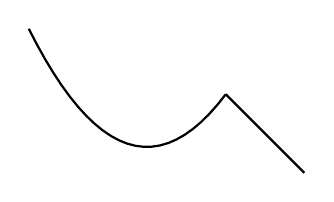
\begin{tikzpicture}
\YEaxis{2}{2}
\YExcoord{1}{2}
\draw [thick] plot[domain=-1.5:1](\x,{\x*\x/1.5+.33});
\draw [thick] plot[domain=1:2](\x,{-\x+2});
\end{tikzpicture}
\end{center}
\end{answer}
\begin{solution}
By Theorem~\ref*{thm:APPlocalMaxMin}, if $x=2$ not a critical point, then it must be a singular point. That is, $f(x)$ is not differentiable at $x=2$. Also, remember that endpoints are not local extrema. Two possibilities are shown below, but there are infinitely many possible answers.
\begin{center}
\begin{tikzpicture}
\YEaxis{2}{2}
\YExcoord{1}{2}
\draw [thick] (-2,1)--(2,1);
\draw  (1,1) node[opendot]{};
\draw (1,1.5) node[vertex]{};
\end{tikzpicture}
\hspace{2cm}
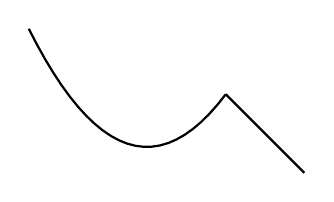
\begin{tikzpicture}
\YEaxis{2}{2}
\YExcoord{1}{2}
\draw [thick] plot[domain=-1.5:1](\x,{\x*\x/1.5+.33});
\draw [thick] plot[domain=1:2](\x,{-\x+2});
\end{tikzpicture}
\end{center}
\end{solution}




\begin{question}
 \[f(x)=\sqrt{\left|(x-5)(x+7)\right|}\]
Find all critical points and all singular points of $f(x)$. You do not have to specify whether a point is critical or singular.
\end{question}
\begin{hint}
You should be able to figure out the global minima of $f(x)$ in your head.
\\
Remember with absolute values, $|X|=\left\{\begin{array}{ll}
X&X\ge0\\
-X&X<0
\end{array}\right.$.
\end{hint}
\begin{answer}
$x=-7$, $x=-1$, and $x=5$
\end{answer}
\begin{solution}
Critical points are those values of $x$ for which $f'(x)=0$, and
singular points are those values of $x$ for which $f(x)$ is not differentiable.
So, we ought to find $f'(x)$. Since $f(x)$ has an absolute value sign, let's re-write it in a version that is friendlier to differentiation. Remember that $|X|=X$ when $X \geq 0$, and $|X|=-X$ when $X<0$.
\begin{align*}
f(x)&=\sqrt{\left|(x-5)(x+7)\right|}\\
&=\left\{\begin{array}{cc}
\sqrt{(x-5)(x+7)}&\mbox{ if } (x-5)(x+7)\ge0\\
\sqrt{-(x-5)(x+7)}&\mbox{ if } (x-5)(x+7)<0
\end{array}\right.
\intertext{The product $(x-5)(x+7)$ is positive when $(x-5)$ and $(x+7)$ have the same sign, and negative when they have opposite signs, so}
f(x)&=\left\{\begin{array}{ll}
\sqrt{(x-5)(x+7)}&\mbox{ if } x\in (-\infty,-7] \cup [5,\infty)\\
\sqrt{-(x-5)(x+7)}&\mbox{ if } x\in(-7,5)
\end{array}\right.
\intertext{Now, when $x \neq -7,5$, we can differentiate, using the chain rule.}
f'(x)&=\left\{\begin{array}{ll}
\frac{\diff{}{x}\left\{(x-5)(x+7)\right\}}{2\sqrt{(x-5)(x+7)}}&\mbox{ if } x\in (-\infty,-7) \cup (5,\infty)\\
\frac{\diff{}{x}\left\{-(x-5)(x+7)\right\}}{2\sqrt{-(x-5)(x+7)}}&\mbox{ if } x\in(-7,5)\\
?? & \mbox{ if } x=-7,\,x=5
\end{array}\right.\\
&=\left\{\begin{array}{ll}
\frac{2x+2}{2\sqrt{(x-5)(x+7)}}&\mbox{ if } x\in (-\infty,-7) \cup (5,\infty)\\
\frac{-2x-2}{2\sqrt{-(x-5)(x+7)}}&\mbox{ if } x\in(-7,5)\\
?? & \mbox{ if } x=-7,\,x=5
\end{array}\right.
\end{align*}
We are tempted to say that the derivative doesn't exist when $x=-7$ and $x=5$, but be careful-- we don't actually know that yet. The formulas we have for the $f'(x)$ are only good when $x$ is \emph{not} $-7$ or $5$.

The middle formula $\dfrac{-2x-2}{2\sqrt{-(x-5)(x+7)}}$ tells us $x=-1$ is a critical point: when $x=-1$, $f'(x)$ is given by the middle line, and it is 0. Note that $x=-1$ also makes the top formula 0, but $f'(-1)$ is not given by the top formula, so that doesn't matter.

What we've concluded so far is that $x=-1$ is a critical point of $f(x)$, and $f(x)$ has no other critical points or singular points when $x \neq -7,5$. It remains to figure out what's going on at $-7$ and $5$. One way to do this is to use the definition of the derivative to figure out what $f'(-7)$  and $f'(5)$ are, if they exist. This is somewhat laborious. Let's look for a better way.

\begin{itemize}
\item First, let's notice that $f(x)$ is defined for all values of $x$, thanks to that handy absolute value sign.
\item Next, notice $f(x) \geq 0$ for all $x$, since square roots never give a negative value.
\item Then if there is some value of $x$ that gives $f(x)=0$, that $x$ gives a global minimum, and therefore a local minimum.
\item $f(x)=0$ exactly when $(x-5)(x+7)=0$, which occurs at $x=-7$ and $x=5$
\item Therefore, $f(x)$ has global and local minima at $x=-7$ and $x=5$
\item So, $x=-7$ and $x=5$ are critical points or singular points by Theorem~\ref*{thm:APPlocalMaxMin}.
\end{itemize}

So, all together:

$x=-1$ is a critical point, and $x=-7$ and $x=5$ are critical points or singular pints (but we don't know which).

Remark: if you would like a review of how to use the definition of the derivative, below we show that $f(x)$ is not differentiable at $x=-7$. (In fact, $x=-7$ and $x=5$ are both singular points.)

\begin{align*}
f'(-7)&=\lim_{h \to 0} \frac{f(-7+h)-f(-7)}{h}\\
&=\lim_{h \to 0} \frac{\sqrt{|(-13+h)(h)|}-\sqrt{|0|}}{h}\\
&=\lim_{h \to 0} \frac{\sqrt{|(-13+h)(h)|}}{h}
\intertext{Let's first consider the case $h>0$.}
\lim_{h \to 0^+} \frac{\sqrt{|(-13+h)(h)|}}{h}&=\lim_{h \to 0^+}\frac{\sqrt{(13-h)(h)}}{h}\\
&=\lim_{h \to 0^+}\frac{\sqrt{13h-h^2}}{\sqrt{h^2}}\\
&=\lim_{h \to 0^+}\sqrt{\frac{13h-h^2}{h^2}}\\
&=\lim_{h \to 0^+}\sqrt{\frac{13}{h}-1}\\
&=\infty
\intertext{Since one side of the limit doesn't exist,}
\lim_{h \to 0} \frac{f(-7+h)-(-7)}{h}&=DNE
\intertext{so $f'(x)$ is not differentiable at $x=-7$. Therefore, $x=-7$ is a singular point.}
\end{align*}
\end{solution}


\begin{question}
Suppose $f(x)$ is the constant function $f(x)=4$. What are the critical points and singular points of $f(x)$? What are its local and global maxima and minima?
\end{question}
\begin{hint}
Review the definitions of critical points and extrema: Definition~\ref*{def:APPcriticalPoint}
and
Definition~\ref*{def:APPlocalMaxMin}.
\end{hint}
\begin{answer}
Every real number $c$ is a critical point of $f(x)$, and $f(x)$ has a local and global maximum and minimum at $x=c$. There are no singular points.
\end{answer}
\begin{solution}
For any real number $c$, $c$ is in the domain of $f(x)$ and $f'(c)$ exists and is equal to zero. So, following
Definition~\ref*{def:APPcriticalPoint}, every real number is  a critical point of $f(x)$, and $f(x)$ has no singular points.

For every number $c$, let $a=c-1$ and $b=c+1$, so $a<c<b$. Then $f(x)$ is defined for every $x$ in the interval $[a,b]$, and
$f(x) =f(c)$ for every $a \le x \le b$. That means $f(x) \leq f(c)$ and $f(x) \geq f(c)$. So, comparing with Definition~\ref*{def:APPlocalMaxMin}, we see that $f(x)$ has a global and local maximum AND minimum at every real number $x=c$.
\end{solution}
